\documentclass[10pt]{article}
\usepackage{graphicx, fancyhdr, enumerate}
\usepackage{amsmath, amsfonts, color, multicol, mathtools}
\usepackage{blkarray}

\setlength{\topmargin}{-.55 in} 
\setlength{\textheight}{9 in}
\setlength{\textwidth}{6.625 in} 
\setlength{\evensidemargin}{-.0625 in}
\setlength{\oddsidemargin}{-.0625 in} 
\setlength{\parindent}{0 in}
\setlength{\headheight}{18.0pt}
\newcommand{\ds}{\displaystyle}
\newcommand{\xbar}{\overline{X}}

\DeclarePairedDelimiter{\ceil}{\lceil}{\rceil}

\cfoot{\thepage} 
\renewcommand{\headrulewidth}{0.4pt} 
\renewcommand{\footrulewidth}{0pt} 
\newcommand{\ansfont}[1]{{\textcolor{blue}{\textbf{Answer:}}\ \ #1}}


\lhead{\Large\sffamily Stat 330 (Fall 2016): Homework 1} 
\rhead{\sffamily Due: August 31, 2016}

% Uncomment the following line to remove answers, and comment line out to show answers:
\renewcommand{\ansfont}[1]{}


\begin{document}
\pagestyle{fancy} 
Show all of your work, and \emph{please} staple your assignment if you use more than one sheet. Write your name, the course number and the section on every sheet. 

\begin{enumerate} 
  \item A coin is tossed three times, and the sequence of heads and tails is recorded.
    \begin{enumerate}
      \item Determine the sample space, $\Omega$.
      \item List the elements that make up the following events: i. $A$ = at least two heads,
        ii. $B$ = the first two tosses result in heads, iii. $C$ = the last toss results in a tail
      \item List the elements of the following events: i. $\overline{A}$, ii. $A\cap C$. iii. $A \cup C$
    \end{enumerate}
    \ansfont{
      \begin{enumerate}
        \item Let $H$ and $T$ stand for the events of head and tail, respectively. \emph{Ergo}, the sample space is
          $$\Omega=\{HHH, HHT, HTH, HTT, THH, THT, TTH, TTT\}$$
        \item \begin{enumerate}
            \item $A=\text{at least two heads}=\{HHH, HHT, THH, HTH\}$
            \item $B=\text{the first two tosses result in heads}=\{HHT, HHH\}$
            \item $C=\text{the last toss results in a tail}=\{HHT, HTT, THT, TTT\}$
          \end{enumerate}
        \item \begin{enumerate}
            \item $\bar{A}=\Omega\setminus A=\{HTT, THT, TTH, TTT\}=\text{at most one head}$
            \item $A\cap C=\{HHT\}$
            \item $A\cup C=\{HHH, HHT, THH, HTH, HTT, THT, TTT\}=$ at least two heads or the last toss results in a tail
          \end{enumerate}
      \end{enumerate}
    }

  \item
    Driving to work, a commuter passes through a sequence of three
    intersections with traffic lights. At each light, she either stops, $s$, or continues, $c$.
    \begin{enumerate}
      \item % Rice 1.2 Ex A 
        \label{lights}
        Determine the set of possible outcomes in the sample space.
        \emph{Notation: use `$csc$' to denote the outcome where she must stop only at the second traffic light.}



      \item % my addition, cont.
        If each of the outcomes is equally likely in (\ref{lights}), then
        what is the probability (or chance) that she doesn't have to stop at any of these lights?
        Comment if  this value seems reasonable to you.

      \item \label{eventlights}
        Let $A$ be an event in the sample space defined in problem (\ref{lights}),
        and have event $A$ be the commuter stops at the first light.
        Let $B$ be the event in (\ref{lights}) that the commuter stops at the second light.
        Following the above notation, list the outcomes in each event:
        \begin{enumerate}
          \item $A$
          \item $B$
          \item $\bar{B}$
          \item $A \cup B$
          \item $A \cap B$
          \item $A \cap \bar{B}$
        \end{enumerate}
    \end{enumerate}
    \ansfont{
      \begin{enumerate}
          %Denote $csc$ as the outcome where she must stop only at the second traffic light.
        \item Following the above notation, the set of all outcomes is
          \[\Omega = \{ccc, ccs, css, csc, sss, ssc, scc, scs\}.\]
        \item
          The outcome of her not stopping at any light is $ccc$. This is one outcome
          out of the possible 8, so the probability of this is 
          \[P(\{ccc\}) = \frac{\mathcal{N}_F}{\mathcal{N}_T}=\frac18.
          \]
          This probability (.125) is reasonable--it's the value if stopping at any light is independent
          of any of the others. In perspective, a value of .95 or .01 would seem unreasonable.
        \item
          \begin{enumerate}
            \item
              {$A=\{sss, ssc, scc, scs\}$.}
            \item
              {$B=\{sss, ssc, css, csc\}$.}
            \item
              {$\bar{B}=\Omega\setminus B = \{ccc, ccs, scc, scs\}$.}
            \item
              {$A\cup B=\{sss, ssc, scc, scs, css, csc\}$.}
            \item
              {$A\cap B=\{sss, ssc\}$.}
            \item
              {$A\cap \bar{B}=\{scc, scs\}$.}
          \end{enumerate}
      \end{enumerate}
    }

  \item Two fair dice are tossed and the number on each die is recorded, e.g. (3,2) indicates the first die had a 3 and the second die had a 2. 
    \begin{enumerate}
      \item Determine the sample space (Hint: there are 36 outcomes.).
      \item What is the probability that the sum of the two numbers is 1?
      \item What is the probability that the sum is 6?
      \item What is the probability that the minimum of the two numbers is 3?
    \end{enumerate}
    \ansfont{
      \begin{enumerate}
        \item The sample space is
          $\{(i,j)| i=1,\dots,6, j=1,\dots,6\}$. That means
          \begin{center}
            $\{ (1,1), (1,2), (1,3), (1,4), (1,5), (1,6),$\\
            $ (2,1), (2,2), (2,3), (2,4), (2,5), (2,6),$\\
            $ (3,1), (3,2), (3,3), (3,4), (3,5), (3,6),$\\
            $ (4,1), (4,2), (4,3), (4,4), (4,5), (4,6),$\\
            $ (5,1), (5,2), (5,3), (5,4), (5,5), (5,6),$\\
            $ (6,1), (6,2), (6,3), (6,4), (6,5), (6,6)\}$.
          \end{center}
        \item The smallest value of the sum is 2 which is obtained by (1,1). Thus, the probability that the sum is 1 is 0.
        \item The corresponding sums of each outcome is
          \begin{center}
            \begin{tabular}{c|cccccc}
              & 1 & 2 & 3 & 4 & 5 & 6\\\hline
              1 & 2 & 3 & 4 &5 & 6 & 7\\
              2 & 3 & 4 & 5 & 6 & 7 & 8\\ 
              3 & 4 & 5 & 6 & 7 & 8 & 9\\ 
              4 & 5 & 6 & 7 & 8 & 9 & 10\\ 
              5 & 6 & 7 & 8 & 9 & 10 & 11\\ 
              6 & 7 & 8 & 9 & 10 & 11 & 12
            \end{tabular}
          \end{center}
          There are five 6s and thus there are 5 outcomes (out of 36 possible outcomes)
          that have sum as 6. The
          required probability is 5/36.
        \item The corresponding minimum of each outcome is
          \begin{center}
            \begin{tabular}{c|cccccc}
              & 1 & 2 & 3 & 4 & 5 & 6\\\hline
              1 & 1 & 1 & 1 & 1 & 1 & 1\\
              2 & 1 & 2 & 2 & 2 & 2 & 2\\ 
              3 & 1 & 2 & 3 & 3 & 3 & 3\\ 
              4 & 1 & 2 & 3 & 4 & 4 & 4\\ 
              5 & 1 & 2 & 3 & 4 & 5 & 5\\ 
              6 & 1 & 2 & 3 & 4 & 5 & 6
            \end{tabular}
          \end{center}
          There are seven 3s and thus there are 7 outcomes (out of 36 possible outcomes)
          that have minimum as 3. The
          required probability is 7/36.
      \end{enumerate}
    }
    
\item
  Out of a group of 40 students all play at least one of badminton, volleyball or table tennis.
  \begin{itemize}
    \item 8 students play all three games, 10 students play badminton and table tennis.
    \item 20 students play table tennis and volleyball, 12 students play badminton and volleyball.
    \item 30 students play table tennis, 25 students play volleyball.
  \end{itemize}
  \begin{enumerate}
    \item
      Draw a Venn diagram of the situation.
    \item
      How many of the students play \emph{only} badminton?
    \item
      How many of the students play badminton?
    \item \label{marginal}
      Assume one student is picked at random from the group.\\
      What is the probability he/she plays badminton?
    \item \label{conditional}
      Assume one student is picked at random from those that play voleyball.\\
      What is the probability he/she plays badminton?
    \item
      Why is the probability that the student is a badminton player different in \ref{marginal} and \ref{conditional}?
  \end{enumerate}

% SOLUTION 3
\ansfont{
  \begin{enumerate}
    \item
      \centerline {
        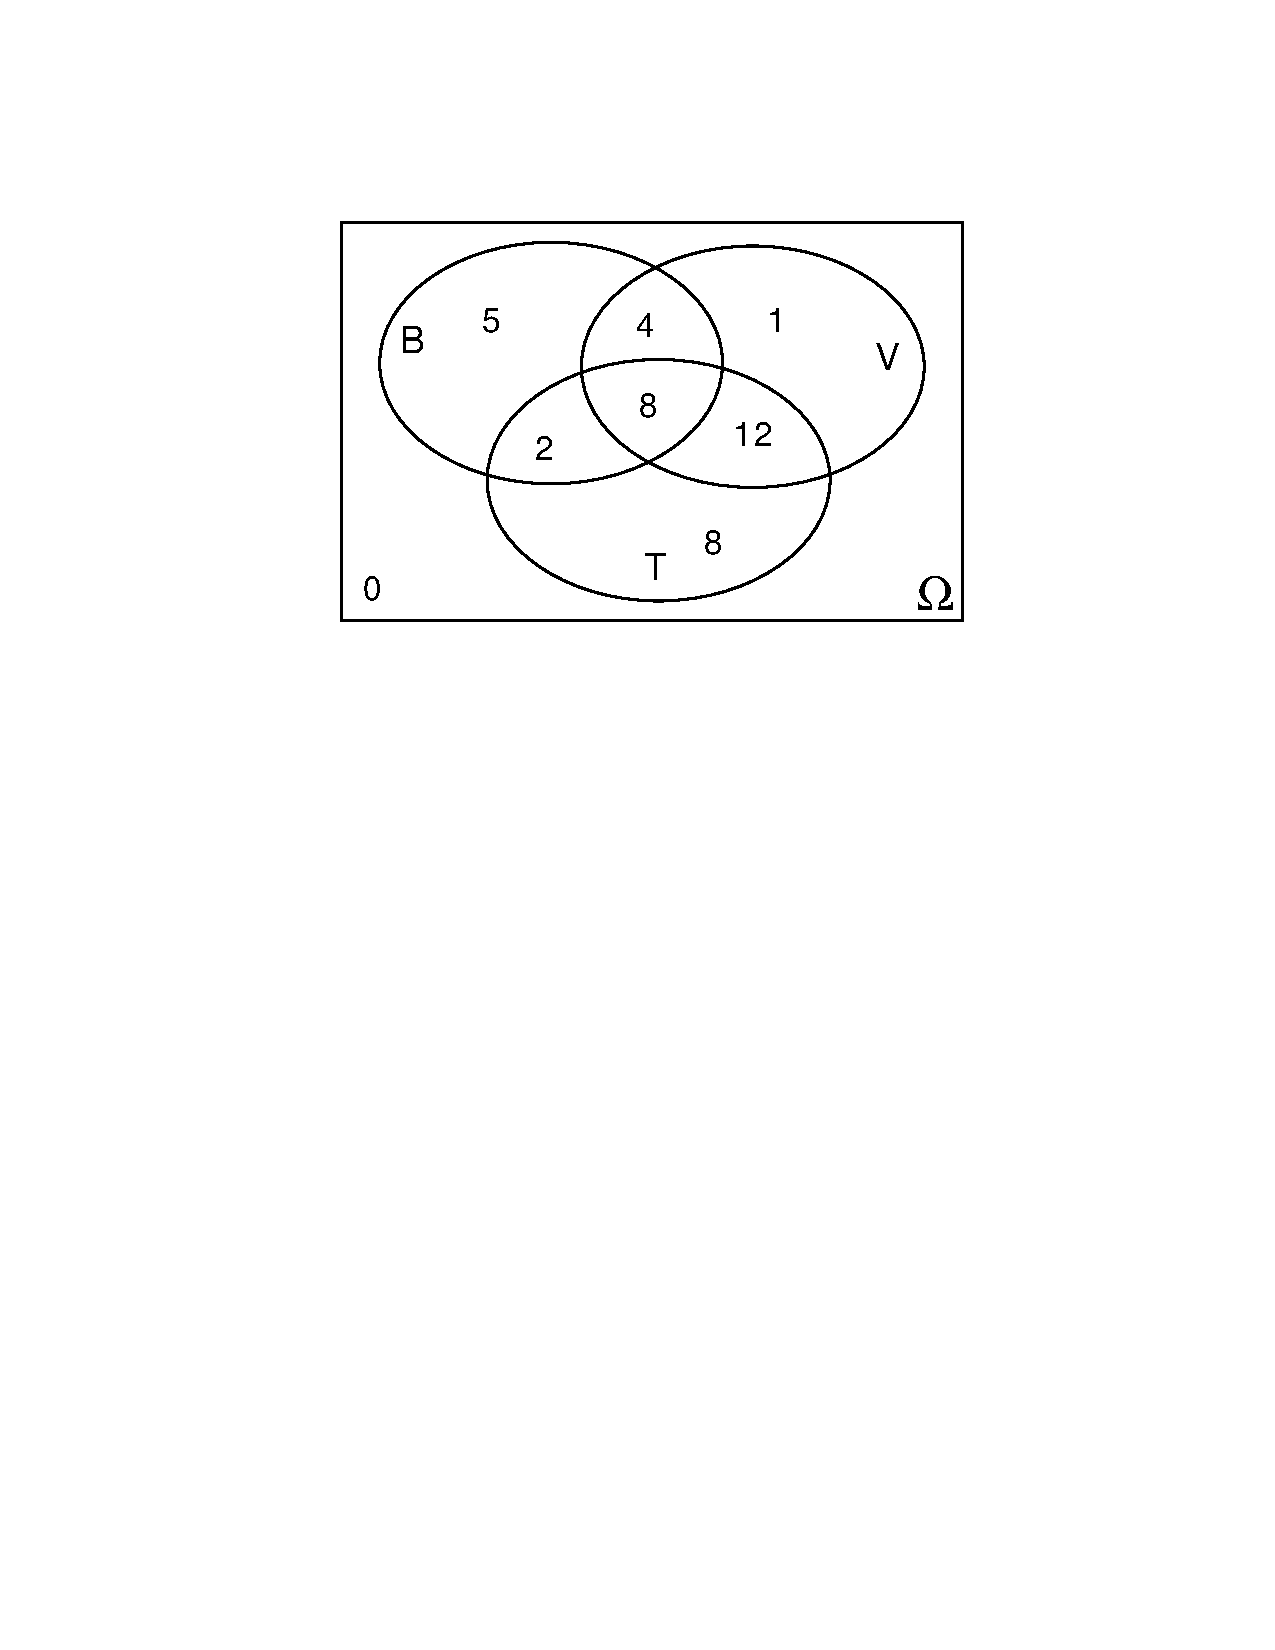
\includegraphics[width=2in]{venn-diagram}
      }
      \vspace{.2in}
    \item 5 students only play badminton.
    \item 5 + 4 + 8 + 2 = 19 students play badminton.
    \item $\frac{\textrm{\# students that play badminton}}{\textrm{total \# students}} = \frac{19}{40}$.
    \item $\frac{\textrm{\# students that play badminton and voleyball}}{\textrm{\# students that play voleyball}} = \frac{4 + 8}{25} = \frac{12}{25}$.
    \item The sample space has effectively been reduced from $\Omega$ down to $V$, where $V$ is the set of students that play voleyball. The proportion of the original 40 students that play badminton is not the same as the proportion of voleyball-playing students who play badminton.
  \end{enumerate}
}
    
    
    
  \item (Baron's book): 2.4
    \ansfont{
      \newline
      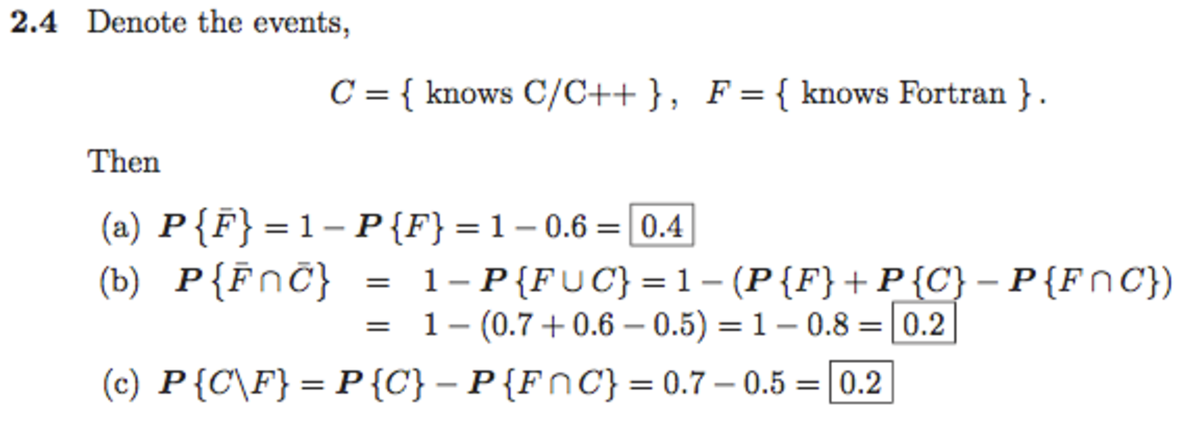
\includegraphics[width=13cm]{baron2-4-1}
      \newline
      \hspace*{1cm}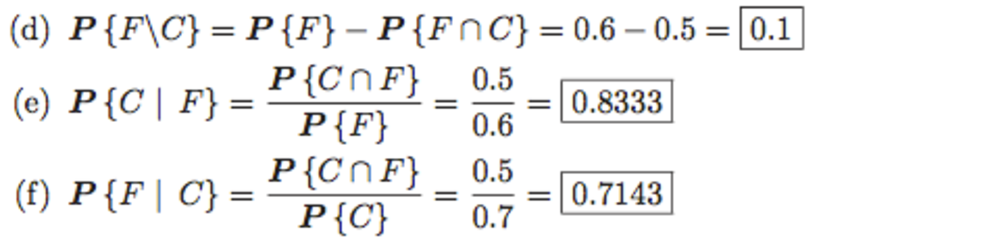
\includegraphics[width=11cm]{baron2-4-2}
    }
  \item (Baron's book): 2.11
    \ansfont{
      \newline
      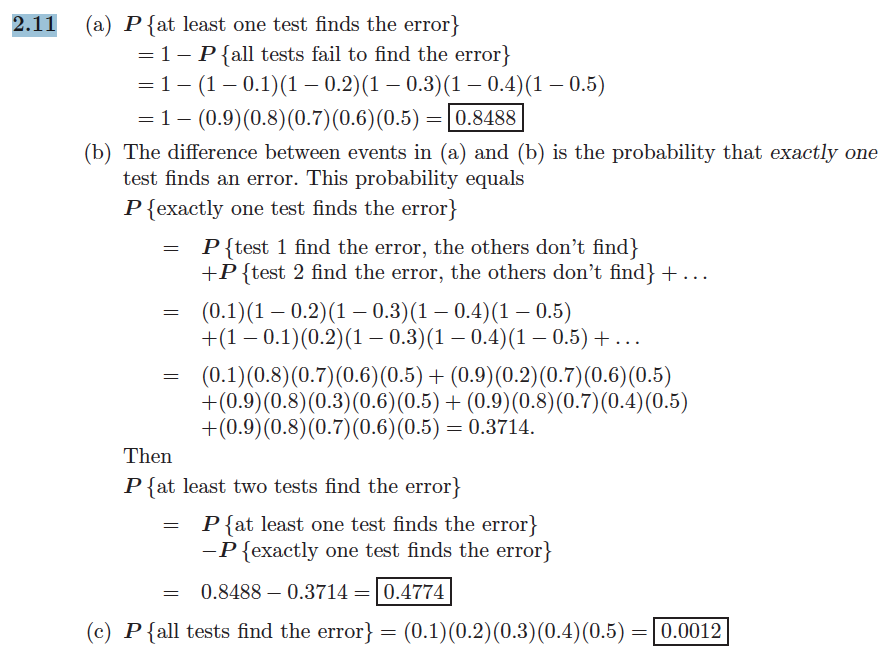
\includegraphics[width=13cm]{baron2-11}
    }
\end{enumerate}
\end{document}
